\documentclass[12pt,a4paper]{article}
\usepackage[utf8]{inputenc}
\usepackage[T1]{fontenc}
\usepackage[spanish]{babel}
\usepackage{geometry}
\geometry{a4paper, margin=1.8cm}
\usepackage{array}
\usepackage{booktabs}
\usepackage{tabularx}
\usepackage{hyperref}
\usepackage{xcolor}
\usepackage{float}
\usepackage{listings}
\usepackage{graphicx}
\usepackage{float}
\usepackage{gensymb}

\hypersetup{
    colorlinks=true,
    linkcolor=blue,
    filecolor=magenta,
    urlcolor=blue,
    pdftitle={Protocolo de Comunicacion BLE - AttaBot STEM},
}

% ----- Estilo para bloques de código -----
\definecolor{codebg}{RGB}{245,245,245}
\definecolor{codegreen}{RGB}{0,110,40}
\definecolor{codeblue}{RGB}{0,60,200}

\lstdefinestyle{cppstyle}{
    backgroundcolor=\color{codebg},
    commentstyle=\color{codegreen},
    keywordstyle=\color{codeblue}\bfseries,
    stringstyle=\color{purple},
    basicstyle=\ttfamily\footnotesize,
    breaklines=true,
    frame=single,
    language=C++,
    showstringspaces=false,
    tabsize=2,
    columns=fullflexible,
    captionpos=b
}
\lstset{style=cppstyle}
\renewcommand{\lstlistingname}{Fragmento de código}

\title{\textbf{Protocolo de Comunicación BLE \\ \large Aplicación -- Robot Atta-Bot STEM}}
\author{AttaBot STEM}
\date{\today}

\begin{document}
\maketitle

Este documento describe algunos conceptos del protocolo de comunicación utilizado entre la aplicación (App) y el robot Atta-Bot STEM. La primera etapa abarca el enlace mediante Bluetooth Low Energy (BLE) entre la aplicación (Central/Client) y el microcontrolador ESP32 del robot (Periférico/Server), implementado mediante la biblioteca nativa \texttt{BLEDevice} del core \texttt{esp32:esp32}. La segunda etapa describe el formato y significado de los comandos que viajan sobre ese enlace, definidos en el protocolo de instrucciones propio del proyecto.

El objetivo es ofrecer una referencia para que al revisar el código fuente (CodigoESP32.ino) se puede reconocer con facilidad qué representa cada línea relacionada con la comunicación. Las fuentes completas utilizadas como base para la construcción del protocolo se encuentran en el apartado de referencias [\ref{sec:referencias}].

\section{Conceptos básicos de BLE}
\label{sec:conceptos}

La siguiente tabla resume conceptos utilizados en este proyecto:

\begin{figure}[H]
    \centering
    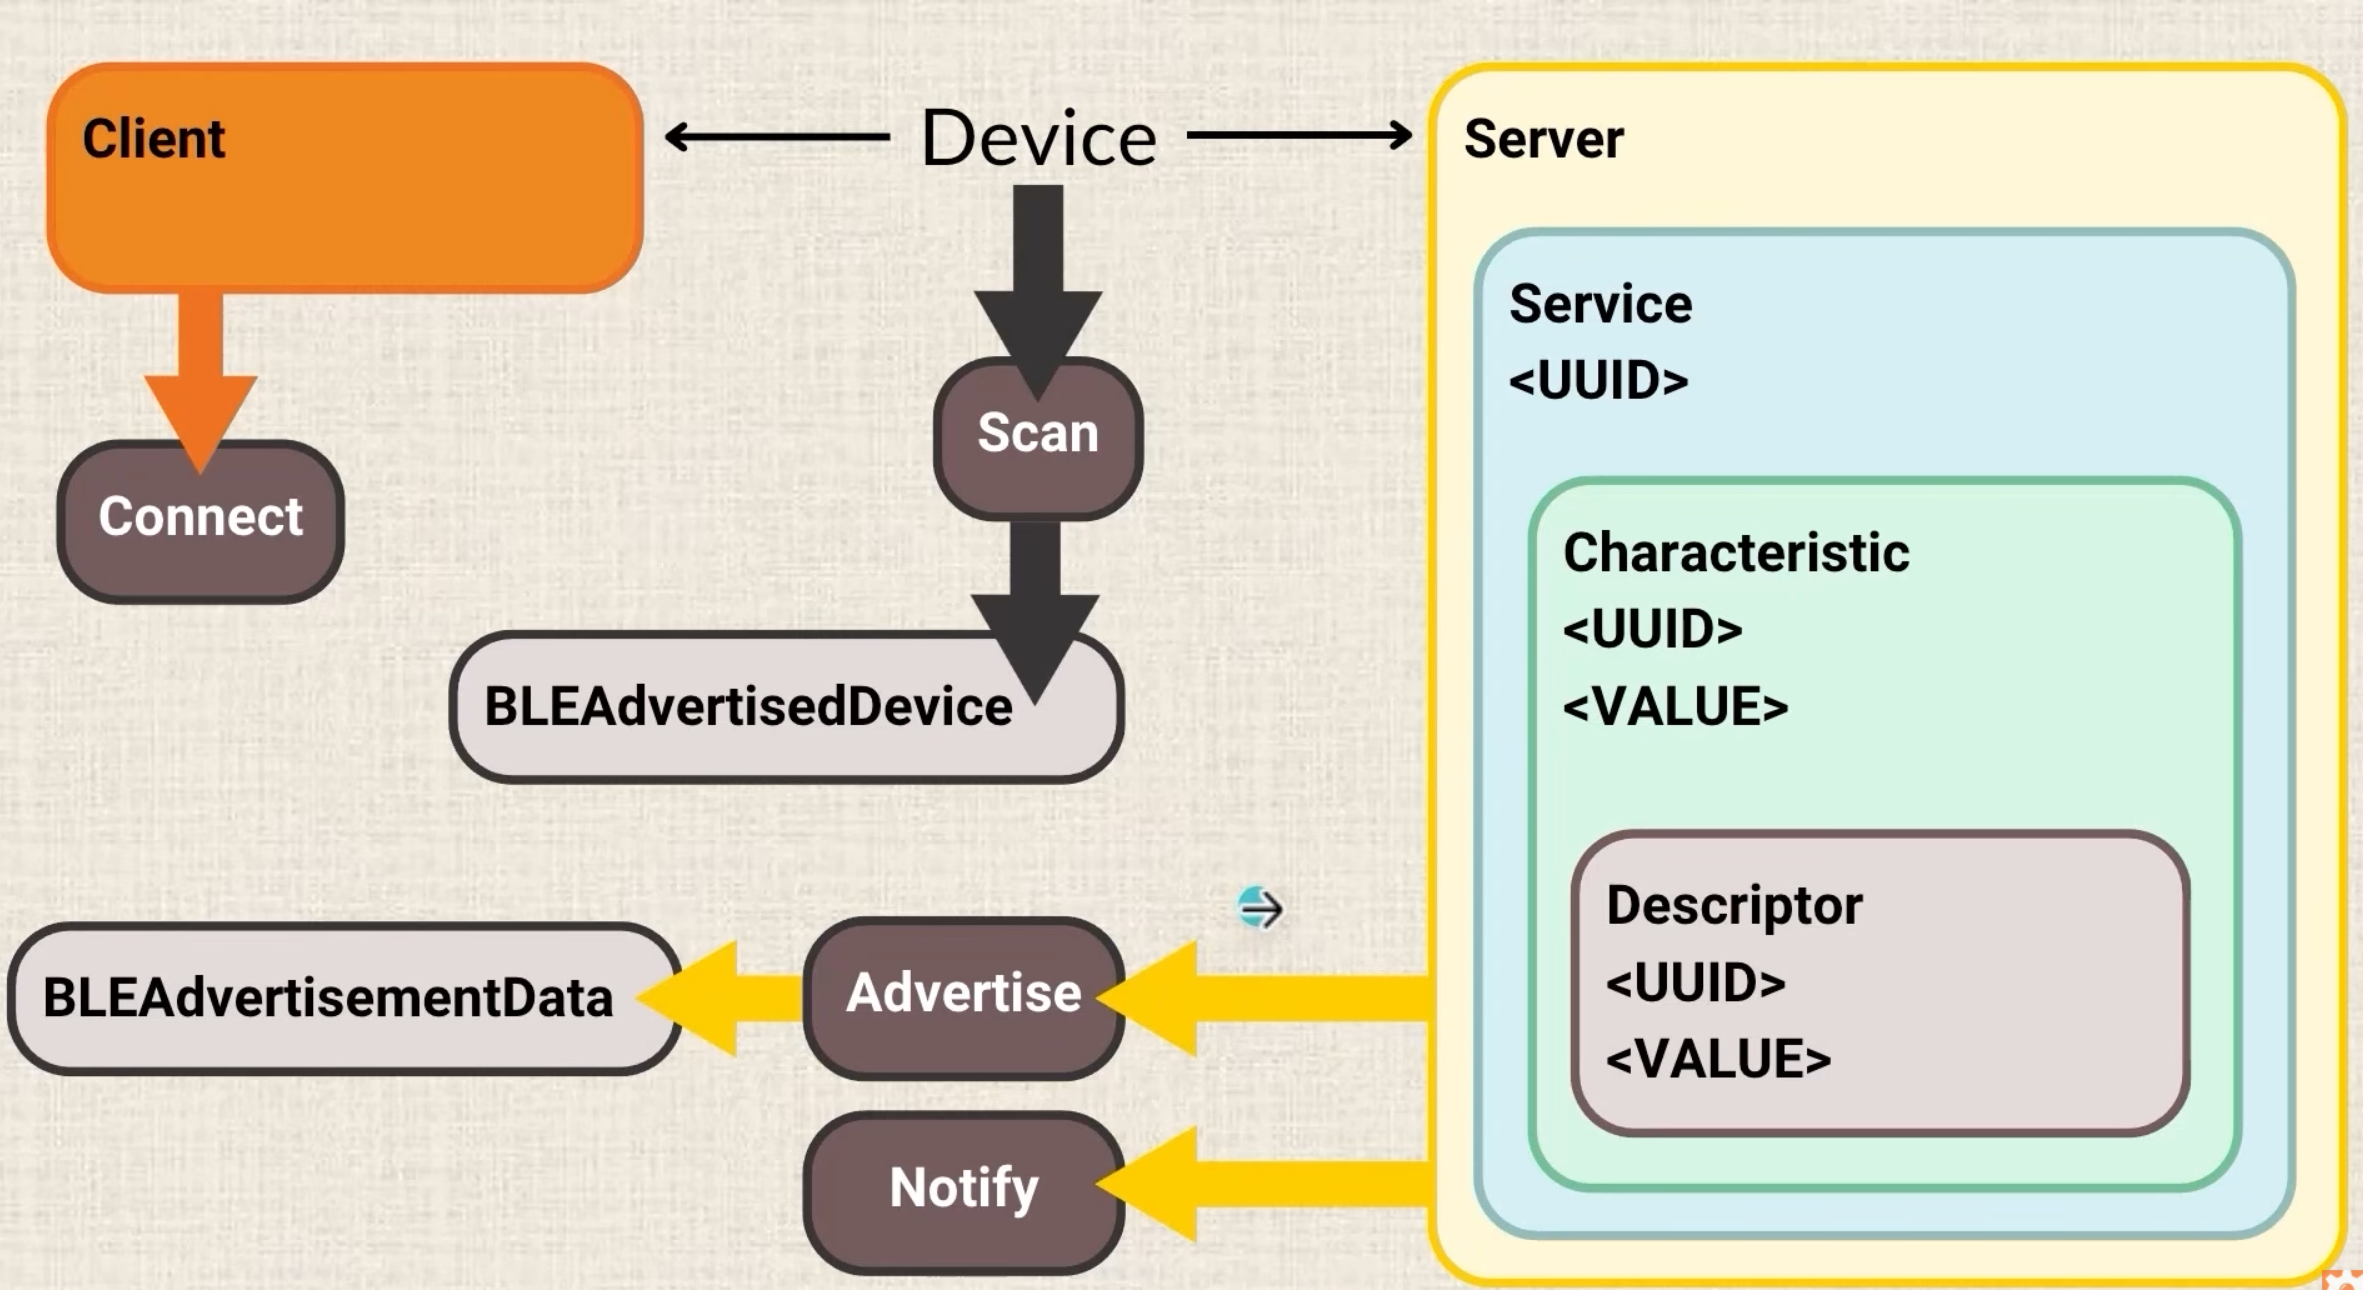
\includegraphics[width=0.6\linewidth]{ReferenceImageBLE.png}
    \caption{Diagrama de Flujo de Comunicación BLE. Tomado de \cite{pea_esp32_ble}.}
    \label{fig:flujo_ble} 
\end{figure}

\begin{table}[H]
    \centering
    \renewcommand{\arraystretch}{1.3}
    \begin{tabularx}{\textwidth}{@{} >{\raggedright\arraybackslash}p{3.6cm} X @{}}
        \toprule
        \textbf{Concepto BLE} & \textbf{Dónde aparece en el código y qué significa} \\
        \midrule
        Inicialización del stack &
        Enciende el controlador Bluetooth del ESP32 y define el nombre con el que el dispositivo será visible al escanear. En el código: \texttt{BLEDevice::init()}. \\
        \addlinespace
        Rol de Periférico/Server &
        El ESP32 actúa como el dispositivo que espera conexiones, en lugar de buscarlas activamente. En el código: \texttt{BLEServer}, \texttt{BLEDevice::createServer()}. \\
        \addlinespace
        Callback de conexión &
        Función que la pila BLE ejecuta automáticamente al conectarse o desconectarse un dispositivo; nunca se llama manualmente. En el código: clase \texttt{BLEServerCallbacks}, métodos \texttt{onConnect()} / \texttt{onDisconnect()}. \\
        \addlinespace
        Servicio &
        Agrupa una o más características bajo un identificador único (UUID); es una categoría dentro de los datos que expone el servidor. En el código: \texttt{BLEService}, \texttt{createService()}. \\
        \addlinespace
        Característico &
        Una pieza de datos específica dentro de un servicio, con su propio UUID, que puede leerse y/o escribirse -- el equivalente a una nota puntual dentro del ``tablero'' de datos del servidor. En el código: \texttt{BLECharacteristic}, \texttt{createCharacteristic()}. \\
        \addlinespace
        Propiedades del característico &
        Determinan qué operaciones puede realizar el dispositivo remoto sobre ese dato: solo lectura, solo escritura, o ambas. En el código: \texttt{PROPERTY\_READ}, \texttt{PROPERTY\_WRITE}. \\
        \addlinespace
        Callback de escritura &
        Se ejecuta automáticamente cuando el dispositivo remoto escribe un nuevo valor en el característico. En el código: clase \texttt{BLECharacteristicCallbacks}, método \texttt{onWrite()}. \\
        \addlinespace
        Advertising (anuncio) &
        Proceso mediante el cual el ESP32 transmite activamente su existencia y disponibilidad para conectarse. Sin este paso, el dispositivo es invisible para cualquier escaneo. En el código: \texttt{getAdvertising()->start()}. \\
        \addlinespace
        \bottomrule
    \end{tabularx}
    \caption{Correspondencia entre conceptos de BLE y elementos del código fuente.}
\end{table}

\section{Arquitectura de implementación en el proyecto}
\label{sec:arquitectura}

El robot utliza un único servicio con un único característico de lectura/escritura, que transporta texto libre. El significado de cada mensaje no lo define BLE, sino el protocolo de aplicación propio del proyecto (Sección~\ref{sec:protocolo}). BLE actúa únicamente como canal de transporte, mientras que la interpretación del contenido ocurre en el firmware, dentro de la función \texttt{Interpreta\_mensajeBLE()}. Cabe destacar que las librerías utilizadas (<BLEDevice.h>, <BLEServer.h>, <BLEUtils.h>) al ser nativas del core \texttt{esp32:esp32} no requieren instalación previa. 

El flujo general de la comunicación se puede sintetizar de la siguiente forma:
Un dispostivo se conecta a un robot Atta. Los avisos de conexión exitosa y recepción de un nuevo comando son detectados con la función \texttt{leerBluetooth()}, la cual revisa variables anidadas a los \textit{callback} definidas por la libería constantemente. Seguidamente la App envía un comando, esto es escribir en el característico con UUID único; ejemplo: ATINIAV300GI090ATFIN - avanzar 300 cm , girar a la izquierda 90\degree. Cuando el mensaje es detectado se llama la función \texttt{Interpreta\_mensajeBLE()} que descompone el mensaje  con una concatenación de condicionales, para así determinar finalmente los siguientes pasos de la máquina de estados general. 

\subsection{Inicialización del servidor BLE}

El siguiente fragmento, tomado de \texttt{setup()}, muestra la creación del servidor, el servicio y el característico:

\begin{lstlisting}[caption={Inicialización BLE en \texttt{setup()}}, label={lst:setup-ble}]
BLEDevice::init("AttaBotSTEM");

pServer = BLEDevice::createServer();
pServer->setCallbacks(new MyServerCallbacks());

BLEService *pService = pServer->createService(
    "4fafc201-1fb5-459e-8fcc-c5c9c331914b");

pCharacteristic = pService->createCharacteristic(
    "beb5483e-36e1-4688-b7f5-ea07361b26a8",
    BLECharacteristic::PROPERTY_READ |
    BLECharacteristic::PROPERTY_WRITE
);
pCharacteristic->setCallbacks(new MyCharacteristicCallbacks());

pService->start();

pServer->getAdvertising()->addServiceUUID(
    "4fafc201-1fb5-459e-8fcc-c5c9c331914b");
pServer->getAdvertising()->start();
\end{lstlisting}

\subsection{Callbacks}

Dado que \texttt{BLEDevice} funciona mediante eventos asíncronos no es posible ``preguntar'' en cada iteración de \texttt{loop()} si llegó un mensaje nuevo, el proyecto define dos clases de callback. La de escritura sobre el característico es la más relevante para el protocolo de mensajes:

\begin{lstlisting}[caption={Callback de escritura sobre el característico}, label={lst:callback-write}]
class MyCharacteristicCallbacks: public BLECharacteristicCallbacks {
    void onWrite(BLECharacteristic *pCharacteristic) {
      String valorRecibido = pCharacteristic->getValue();
      if (valorRecibido.length() > 0) {
        mensajeBLEBuffer = string(valorRecibido.c_str());
        nuevoMensajeBLE = true;
      }
    }
};
\end{lstlisting}

La bandera \texttt{nuevoMensajeBLE} se revisa dentro de \texttt{loop()} (a través de \texttt{leerBluetooth()}) para procesar el mensaje recibido sin depender de un  \textit{polling} constante. La documentación oficial de BLE para ESP32 contiene una explicación y justificación detallada del uso de estas clases \cite{kolban_ble}.

\section{Protocolo de mensajes de la aplicación}
\label{sec:protocolo}


\subsection{Consideraciones generales}
\begin{itemize}
    \item Cada comando enviado tiene una longitud fija de 5 caracteres.
    \item No existen divisores entre comandos (sin comas, espacios, etc.).
    \item Todo mensaje completo inicia con un comando de encabezado y finaliza con un comando de finalización.
\end{itemize}

\subsection{Lista de comandos}

\begin{table}[H]
    \centering
    \renewcommand{\arraystretch}{1.15}
    \begin{tabularx}{\textwidth}{@{} l X @{}}
        \toprule
        \textbf{Comando} & \textbf{Detalles} \\
        \midrule
        \texttt{ATINI} & Encabezado del mensaje con instrucciones \\
        \texttt{ATFIN} & Finalización del mensaje con instrucciones \\
        \texttt{OBINI} & Inicio de la detección de obstáculos \\
        \texttt{OBFIN} & Finalización de la detección de obstáculos \\
        \texttt{CI\#\#\#} & Inicio del ciclo. \texttt{\#\#\#} indica la cantidad de repeticiones \\
        \texttt{CIFIN} & Finalización del ciclo \\
        \texttt{WH\#\#\#} & Inicio del ciclo condicional \textit{while}. \texttt{\#\#\#} indica la condición (Nota 3) \\
        \texttt{WHFIN} & Finalización del ciclo condicional \textit{while} \\
        \texttt{IF\#\#\#} & Inicio de bifurcación \textit{if}. \texttt{\#\#\#} indica la condición (Nota 3) \\
        \texttt{EL\#\#\#} & Inicio de bifurcación \textit{else if}. \texttt{\#\#\#} indica la condición (Nota 3) \\
        \texttt{IFFIN} & Finalización de bifurcación \textit{if} \\
        \texttt{AV\#\#\#} & Avanzar una distancia de \texttt{\#\#\#} cm \\
        \texttt{RE\#\#\#} & Retroceder una distancia de \texttt{\#\#\#} cm \\
        \texttt{GI\#\#\#} & Giro a la izquierda un ángulo de \texttt{\#\#\#} grados \\
        \texttt{GD\#\#\#} & Giro a la derecha un ángulo de \texttt{\#\#\#} grados \\
        \texttt{HEINI} & Inicio del uso del marcador \\
        \texttt{HEFIN} & Finalización del uso del marcador \\
        \texttt{HE\#\#\#} & Activación del servomotor del set de herramienta. \texttt{\#\#\#} indica la acción (Nota 4) \\
        \texttt{ATCOI} & Encabezado del mensaje de control \\
        \texttt{ATCOF} & Finalización del mensaje de control \\
        \texttt{PARAR} & Detener el robot \\
        \texttt{EJECU} & Ejecutar comandos guardados en la memoria del robot \\
        \bottomrule
    \end{tabularx}
    \caption{Lista de comandos del protocolo de instrucciones.}
\end{table}

\textbf{Nota 1.} En todos los comandos con \texttt{\#\#\#}, este representa un número entero de 3 dígitos sin signo.

\textbf{Nota 2.} Los comandos relacionados con instrucciones que el robot debe ejecutar en secuencia se envían dentro de los encabezados de ``mensaje con instrucciones'' (\texttt{ATINI} / \texttt{ATFIN}). Los comandos que deben ejecutarse con prioridad sobre cualquier otra tarea se envían dentro de los encabezados de control (\texttt{ATCOI} / \texttt{ATCOF}).

\textbf{Nota 3.} Para los comandos \texttt{IF}/\texttt{EL} y \texttt{WH}, \texttt{\#\#\#} representa las condiciones de los sensores infrarrojos de seguimiento (\textit{tracker}):

\begin{table}[H]
    \centering
    \renewcommand{\arraystretch}{1.2}
    \begin{tabularx}{0.55\textwidth}{@{} c X X @{}}
        \toprule
        \textbf{Valor \texttt{\#\#\#}} & \textbf{Sensor tracker izquierdo} & \textbf{Sensor tracker derecho} \\
        \midrule
        \texttt{000} & No detecta & No detecta \\
        \texttt{001} & No detecta & Detecta \\
        \texttt{010} & Detecta & No detecta \\
        \texttt{011} & Detecta & Detecta \\
        \bottomrule
    \end{tabularx}
    \caption{Condiciones de sensores para bifurcaciones \texttt{IF} / \texttt{EL}.}
\end{table}

\begin{table}[H]
    \centering
    \renewcommand{\arraystretch}{1.2}
    \begin{tabularx}{0.8\textwidth}{@{} c l X X @{}}
        \toprule
        \textbf{Valor \texttt{\#\#\#}} & \textbf{Tipo de condición} & \textbf{Sensor tracker   izquierdo} & \textbf{Sensor tracker   derecho} \\
        \midrule
        \texttt{100} & Hasta / \textit{WhileNot} & No detecta & No detecta \\
        \texttt{000} & Mientras / \textit{While} & No detecta & No detecta \\
        \bottomrule
    \end{tabularx}
    \caption{Condiciones de sensores para el ciclo \texttt{WH}.}
\end{table}

\textbf{Nota 4.} Para el comando \texttt{HE\#\#\#}, \texttt{\#\#\#} representa una acción:

\begin{table}[H]
    \centering
    \renewcommand{\arraystretch}{1.2}
    \begin{tabularx}{0.3\textwidth}{@{} c X @{}}
        \toprule
        \textbf{Valor \texttt{\#\#\#}} & \textbf{Acción} \\
        \midrule
        \texttt{101} & Abrir garra \\
        \texttt{001} & Cerrar garra \\
        \texttt{102} & Subir grúa \\
        \texttt{002} & Bajar grúa \\
        \bottomrule
    \end{tabularx}
    \caption{Acciones para el comando \texttt{HE\#\#\#}.}
\end{table}


\begin{thebibliography}{00}
\label{sec:referencias}
\bibitem{arduinoble}
Arduino, ``ArduinoBLE Library Reference,'' Arduino Docs. [En línea]. Disponible en: \url{https://docs.arduino.cc/libraries/arduinoble/}. [Accedido: 25-jul-2026].

\bibitem{kolban_ble}
N. Kolban, ``BLE C++ Guide,'' Repositorio esp32-snippets. [En línea]. Disponible en: \url{https://github.com/nkolban/esp32-snippets/blob/master/Documentation/BLE\%20C++\%20Guide.pdf}. [Accedido: 25-jul-2026].

\bibitem{pea_esp32_ble}
Programming Electronics Academy, ``ESP32 BLE Server + Client,'' YouTube, 21-abr-2025. [Video en línea]. Disponible en: \url{https://www.youtube.com/watch?v=lj99N6pW-Ew&t=742s}. [Accedido: 25-jul-2026].
\end{thebibliography}

\end{document}